\documentclass[9pt]{beamer}

\usetheme{default}

\usepackage{graphicx}
\usepackage{booktabs}
\usepackage{array}
\usepackage{paralist}
\usepackage{verbatim}
\usepackage{subfig}
\usepackage{amsmath}
\usepackage[none]{hyphenat}

%title page
\title{Twisted bilayer NbSe$_2$}
\subtitle{Semester 1 presentation}
\author{Conan Birkett}
\institute{University of Bath department of Physics}


\begin{document}

\begin{frame}
  \titlepage
\end{frame}

\begin{frame}{Outline}
  \begin{itemize}
      \item Introduction
      \item Modelling NbSe$_2$
      \item Adding a twist
      \item Constructing a heterostructure
      \item What's next?
      \item References
  \end{itemize}
\end{frame}

\begin{frame}{Introduction}
  In 2018 researchers at MIT found evidence of superconductivity in 'magic-angle' twisted bilayer graphene (source). This has led to a wave of research in the field of 'twistronics'.

  This project is on a van der waals heterostructure of twisted bilayer NbSe$_2$
\end{frame}

\begin{frame}{Tight binding model with spin orbit coupling}{Modelling NbSe$_2$}
  For our model of NbSe$_2$ we use a multi-orbital tight binding model from R. Habara and K. Wakabayashi (source). It includes the $d_{z^2}$, $d_{xy}$ and $d_{x^2-y^2}$ orbitals of Nb atoms up to third nearest neighbor sites to describe the electronic states of the NbSe$_2$ monolayer. The eigenvalue equation for the TBM is
  \begin{equation}
    \label{TBM_evalue_eqn}
    \hat{H}(\boldsymbol{k})\left|u_{n k}\right\rangle=E_{n k}\left|u_{n k}\right\rangle
  \end{equation}

  where $k=\left(k_{x}, k_{y}\right)$ is the wave-number vector, $E_{nk}$ is the eigenvalue and $n = 1,2,\cdots,6$ is the band index. The eigenvector is defined as

  \begin{equation}
    \left|u_{n k}\right\rangle=$ $\left(c_{n k, d_{z^{2}}, \uparrow}, c_{n k, d_{x y}, \uparrow}, c_{n k, d_{x^{2}-y^{2}}, \uparrow}, c_{n k, d_{z^{2}}, \downarrow}, c_{n k, d_{x y}, \downarrow}, c_{n k, d_{x^{2}-y^{2}}, \downarrow}\right)^{T}
  \end{equation}

  where $(\cdots)^T$ indicates the transpose of the vector and $c_{nk\tau s}$ is the amplitude at atomic orbital $\tau$ with spin $s$ for the $n$th energy band at $k$.
\end{frame}

\begin{frame}{TBM Hamiltonian}{Modelling NbSe$_2$}
  The Hamiltonian with spin orbit coupling can be written as

  \begin{equation}
    \hat{H}(\boldsymbol{k})=\hat{\sigma}_{0} \otimes \hat{H}_{\mathrm{TNN}}(\boldsymbol{k})+\hat{\sigma}_{z} \otimes \frac{1}{2} \lambda_{\mathrm{SOC}} \hat{L}_{z}
  \end{equation}

  Where we have the tight binding nearest neighbor (NN) Hamiltonian

  \begin{equation}
    \hat{H}_{\mathrm{TNN}}(\boldsymbol{k})=\left(\begin{array}{ccc}
    V_{0} & V_{1} & V_{2} \\
    V_{1}^{*} & V_{11} & V_{12} \\
    V_{2}^{*} & V_{12}^{*} & V_{22}
    \end{array}\right)
  \end{equation}

  and

  \begin{equation}
    \hat{L}_{z}=\left(\begin{array}{ccc}
    0 & 0 & 0 \\
    0 & 0 & -2 i \\
    0 & 2 i & 0
    \end{array}\right)
  \end{equation}

  $\hat{\sigma}_0$ and $\hat{\sigma}_z$ are pauli matrices and $\lambda_{\text{SOC}}=0.0784$ eV is the Ising-type spin orbit coupling parameter. $V_0 \cdots V_{22}$ are functions of $k$(source)
\end{frame}

\begin{frame}{TBM Nearest Neighbors (NN)}{Modelling NbSe$_2$}
  \begin{figure}
    \centering
    \resizebox{6cm}{!}{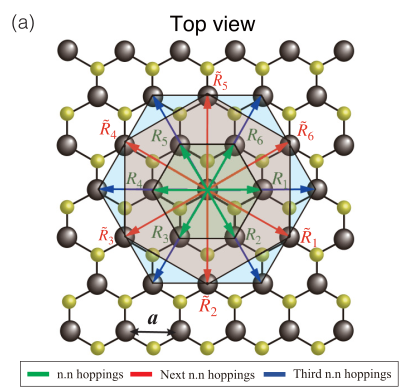
\includegraphics{./Habara_NN.png}}
    \caption{FIG. 1. (a) from Habara et al(source) Displaying a top-down view of the structure of monolayer NbSe$_2$ consisting of Nb (black) and Se(yellow) atoms. The first, second and third nearest neighbor sites are shown in green, red and blue respectively. $a$ is the lattice constant.}
  \end{figure}
\end{frame}

\begin{frame}{1st Brillouin zone (BZ)}{Modelling NbSe$_2$}
  The result is a 6 by 6 Hamiltonian that is a function of wavevector $k$. From our eigenvalue equation \eqref{TBM_evalue_eqn} we can then determine the energy of the 6 electronic (eigen-)states at a given point in $k$-space, specifically, we can take slices in the first brillouin zone along the standard critical points, and even a surface over $k$ space.

  \begin{figure}
    \centering
    \resizebox{4cm}{!}{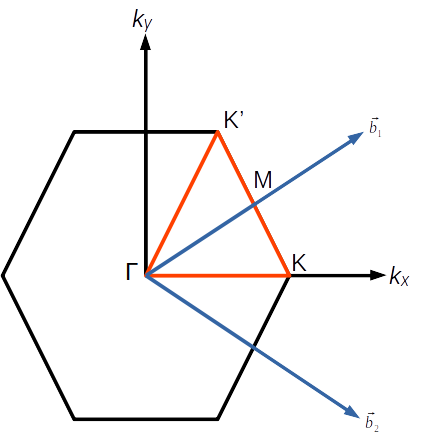
\includegraphics{1st_BZ.png}}
    \caption{The first brillouin zone of the NbSe$_2$ lattice. $\Gamma, K, K' \text{ and } M$ are the standard critical points. $\vec{b_1}, \vec{b_2}$ are the reciprocal lattice vectors, shown in red is the slice $\Gamma \rightarrow K \rightarrow M \rightarrow K' \rightarrow \Gamma$}
  \end{figure}

\end{frame}

\begin{frame}{Electronic band structure}{Modelling NbSe$_2$}
  As a consequence of Bloch's theorem, the eigenstates and their eigenvalues seen in the 1st brillouin zone repeat throughout the lattice. Additionally due to reflectional symmetry in the region to find the energy of the electronic states in can be reduced to the equilateral triangle bounded by $\Gamma \rightarrow K \rightarrow M \rightarrow K' \rightarrow \Gamma$.

  \begin{figure}
  \centering
  \begin{minipage}{.5\textwidth}
    \centering
    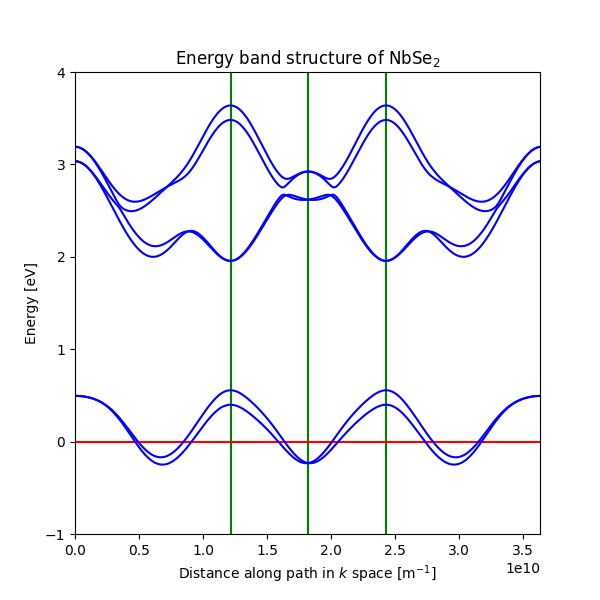
\includegraphics[width=.9\linewidth]{evalues_1.png}
    \captionof{figure}{Energy band structure taken across slice $\Gamma \rightarrow K \rightarrow M \rightarrow K' \rightarrow \Gamma$. Critical points are shown in green and the Fermi level (red) is set to 0 eV}
  \end{minipage}%
  \begin{minipage}{.5\textwidth}
    \centering
    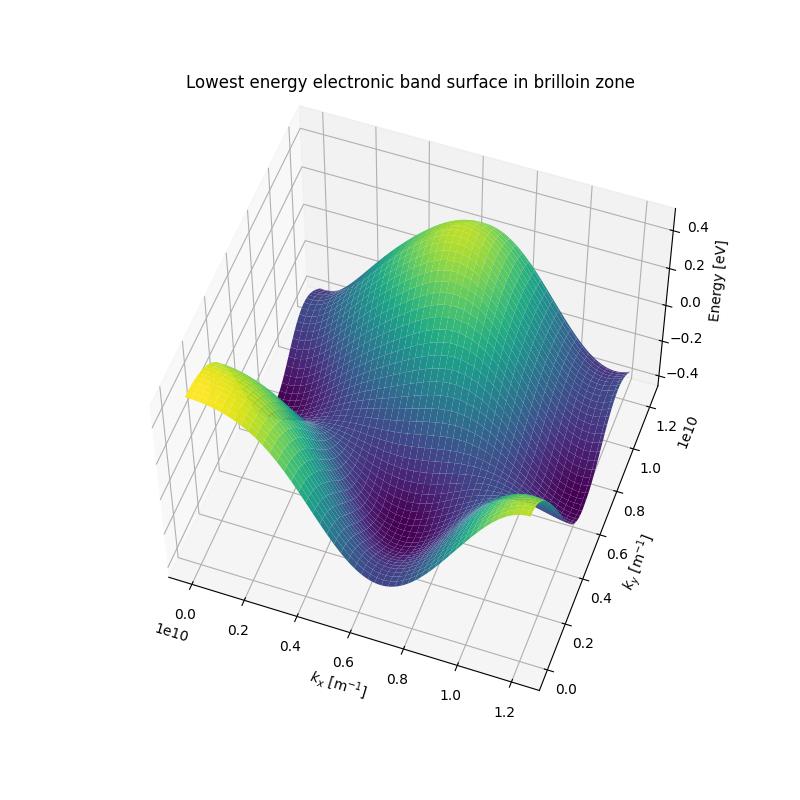
\includegraphics[width=.9\linewidth]{unrotated_surface.png}
    \captionof{figure}{A plot of the surface of the lowest energy state in the same region. The same peaks can be seen at critical points $\Gamma, K, \text{and} K'$}
  \end{minipage}
  \end{figure}
\end{frame}

\begin{frame}{Rotating vectors}{Adding a twist}
  In order to construct a twisted bilayer, we must first figure out how to describe a twisted monolayer. A simple rotation in primitive lattice vectors $a_1, a_2 -> a_1', a_2'$ corresponds to the same rotation in reciprocal lattice vectors $b_1, b_2 -> b_1', b_2'$

  We can consider this a rotation of the whole coordinate system in $k$ space to coordinates in $(k_x', k_y')$. Then all of the physics remains the same

  The result of this is that in order to describe a vector $(k_x', k_y')$ in rotated $k$ space (such as $Gamma, K$ etc) in terms of our unrotated coordinate system $k_x, k_y$ it has to be rotated \textit{inversely} to the rotation of the layer
\end{frame}

\begin{frame}{Twisted surface}{Adding a twist}
  \begin{figure}
    \centering
    \resizebox{8cm}{!}{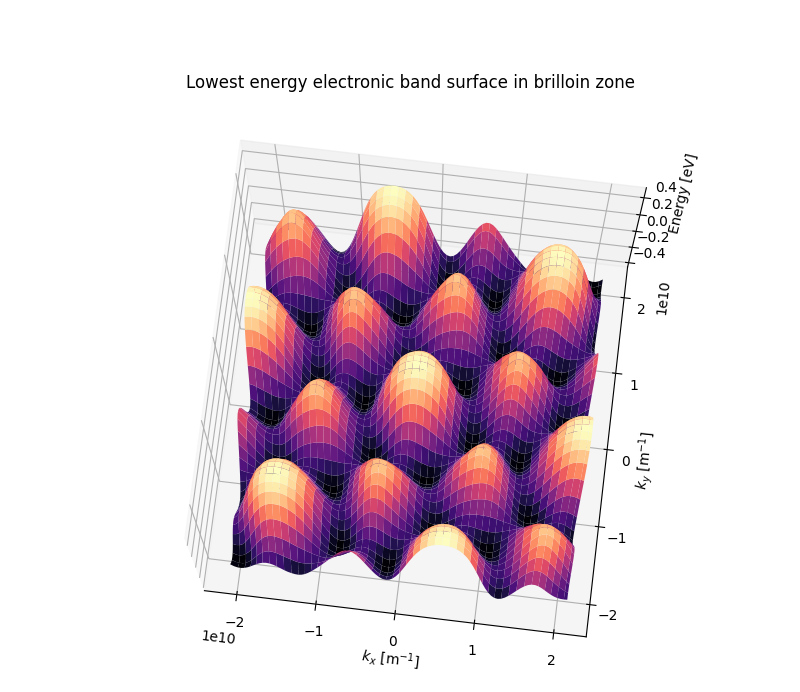
\includegraphics{twisted_mono_surface.png}}
    \caption{A surface of the lowest energy state plotted against unrotated $k_x, k_y$ axes. A twist of 15$^\circ$ is applied to the surface counter clockwise. The plot has been extended to an area encompassing the first brillouin zone to show this more clearly}
  \end{figure}
\end{frame}

\begin{frame}{Heterostructure Hamiltonian}{Constructing a heterostructure}
  Now that we can describe a rotated layer of NbSe$_2$ we can now model two layers at once, with one rotated. A simple model assumes no interaction between states in different layers. We construct a Hamiltonian for the whole system by combining the Hamiltonians of each layer into a 12 by 12 block diagonal matrix

  \begin{equation}
    \hat{H}(\boldsymbol{k})=\left(\begin{array}{cc}
      \hat{H_1}(\boldsymbol{k}) & 0\\
      0 & \hat{H_2}(\boldsymbol{k'})
    \end{array}\right)
  \end{equation}

  Where $\hat{H_1}(\boldsymbol{k})$ and $\hat{H_2}(\boldsymbol{k'})$ are the Hamiltonians of the unrotated and rotated layers respectively. Note that $\hat{H_2}(\boldsymbol{k'})$ is a function of $k'$ which means that an implementation of this matrix of this function must rotate the $k$ input (as described on the previous slide) before it is input into $\hat{H_2}(\boldsymbol{k'})$
\end{frame}

\begin{frame}{Heterostructure eigenvalues}{Constructing a heterostructure}
  \begin{figure}
    \centering
    \resizebox{6cm}{!}{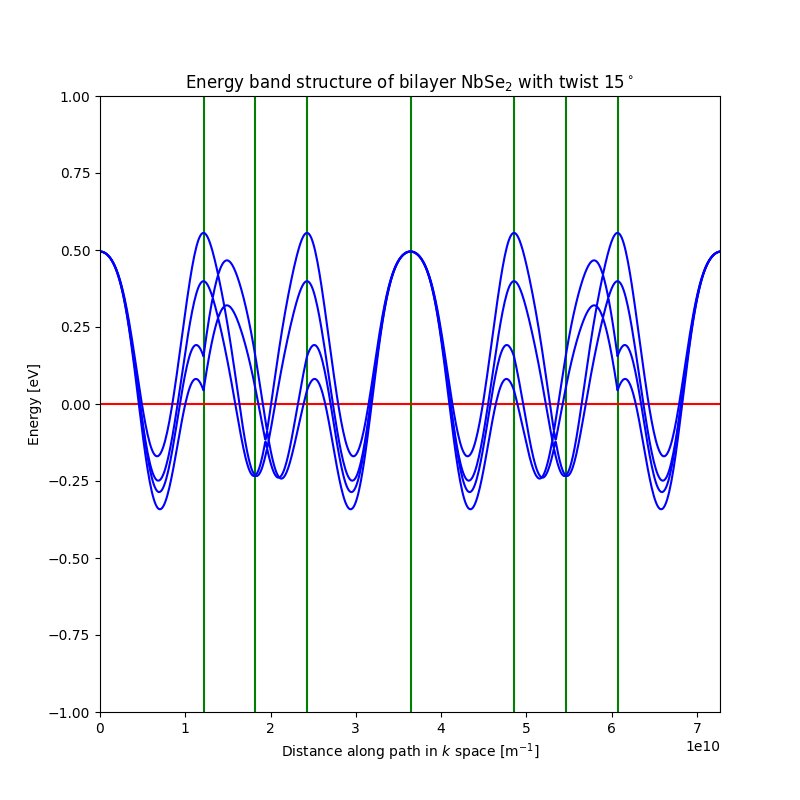
\includegraphics{evalues_2.png}}
    \caption{The four lowest energy eigenvalues of the heterostructure with a twist of 15$^\circ$ applied to the second layer. This plot is taken in the path $\Gamma \rightarrow K \rightarrow M \rightarrow K' \rightarrow \Gamma$ in the unrotated layer and then the same points from the rotated layer. For now, we are only looking at these eigenvalues because they are at the Fermi level, and the corresponding Fermi-surface will describe the electronic properties of the material}
  \end{figure}
\end{frame}

\begin{frame}{Coupling layers - the $d_{z^2}$ orbital}{What's next}
  Currently, we are assuming no interaction between the electronic states on different layers, however looking at the $d$ orbitals that we're modelling with the TBM. the $d_{z^2}$ orbital actually projects out (substantially) in the $z$ axis. Therefore it is a good candidate for describing at inter-layer coupling effects.

  \begin{figure}
    \centering
    \resizebox{4cm}{!}{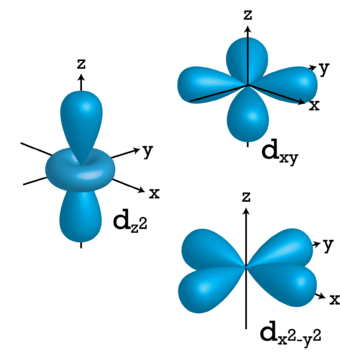
\includegraphics{d_orbitals.png}}
    \caption{Depictions of the $d$ orbitals from lumenlearning.com (source), note the projection of the $d_{z^2}$ orbital into the $z$ axis}
  \end{figure}
\end{frame}

\begin{frame}{Naive steps forwards}{What's next}
  We will make several assumptions regarding the interaction of orbitals between layers. Firstly, that the influence of the $d_{xy}$ and $d_{x^2-y^2}$ orbitals are restricted in to their corresponding $xy$ planes i.e the layers they exist in.

  This leaves the $d_{z^2}$ orbital. There is no quantum process (that we are considering) that will allow for the transition into states of different spin. So we are left with four processes to consider

  \begin{itemize}
    \item $d_{z^2, \downarrow, 1} \rightarrow d_{z^2, \downarrow, 2}$
    \item $d_{z^2, \downarrow, 2} \rightarrow d_{z^2, \downarrow, 1}$
    \item $d_{z^2, \uparrow, 1} \rightarrow d_{z^2, \uparrow, 2}$
    \item $d_{z^2, \uparrow, 2} \rightarrow d_{z^2, \uparrow, 1}$
  \end{itemize}

  where $d_{z^2, s, i}$ is the $d_{z^2}$ orbital with spin $s$ on layer $i$ (we will use $i=2$ as the rotated layer)

  All of these processes should have the same transition energy, the next step is to try and model them
\end{frame}

\begin{frame}{Something interesting}{What's next}

  interesting graph here

\end{frame}

\begin{frame}{References}
  \begin{itemize}
      \item asd
      \item https://courses.lumenlearning.com/cheminter/chapter/orbitals/
  \end{itemize}
\end{frame}

\end{document}
